\documentclass[11pt,a4paper]{article}

% --- Essential Packages ---
\usepackage[a4paper,margin=1in,top=1.2in,bottom=1.1in]{geometry}
\usepackage[utf8]{inputenc}
\usepackage[T1]{fontenc}
\usepackage{lmodern}
\usepackage{amsmath,amssymb}
\usepackage{xcolor}
\usepackage[most]{tcolorbox}
\usepackage{listings}
\usepackage{fancyhdr}
\usepackage{booktabs}
\usepackage{tabularx}
\usepackage{colortbl}
\usepackage{tikz}
\usetikzlibrary{shapes.geometric, arrows.meta, positioning, calc, shadows}
\usepackage{hyperref}
\usepackage{enumitem}
\usepackage{titlesec}

% --- Color Palette (per Report Style Guide) ---
\definecolor{navyHead}{HTML}{1A1A2E}
\definecolor{accentBlue}{HTML}{1F6FB2}
\definecolor{tableHeadNavy}{HTML}{2C3E50}
\definecolor{tableStripe}{HTML}{EAF1F8}
\definecolor{calloutFill}{HTML}{EAF6FB}
\definecolor{calloutBorder}{HTML}{4FA8D8}
\definecolor{codeFill}{HTML}{F6F5F0}
\definecolor{codeBorder}{HTML}{7FB8DE}
\definecolor{codeTab}{HTML}{4FA8D8}
\definecolor{kw}{HTML}{8B008B}
\definecolor{str}{HTML}{B5651D}
\definecolor{cmt}{HTML}{2E8B57}
\definecolor{mintGreen}{HTML}{D9F2E3}
\definecolor{paleSalmon}{HTML}{FBE0DE}
\definecolor{passGreen}{HTML}{2E8B57}
\definecolor{pageBorderColor}{HTML}{D1D5DB}

% --- Diagram Palette ---
\definecolor{uiFill}{HTML}{DCEEFA}
\definecolor{uiBorder}{HTML}{2E75B6}
\definecolor{ctrlFill}{HTML}{E5E5E5}
\definecolor{ctrlBorder}{HTML}{333333}
\definecolor{modelFill}{HTML}{FADBD8}
\definecolor{modelBorder}{HTML}{C0392B}
\definecolor{utilFill}{HTML}{DDF2E3}
\definecolor{utilBorder}{HTML}{27AE60}
\definecolor{dbFill}{HTML}{EAD9F2}
\definecolor{dbBorder}{HTML}{8E44AD}

% --- Hyperref Setup ---
\hypersetup{
    colorlinks=true,
    linkcolor=accentBlue,
    filecolor=accentBlue,
    urlcolor=accentBlue,
    citecolor=accentBlue
}

% --- Heading Typography ---
\titleformat{\section}
  {\color{navyHead}\normalfont\Large\bfseries}{\thesection}{1em}{}
\titleformat{\subsection}
  {\color{accentBlue}\normalfont\large\bfseries}{\thesubsection}{1em}{}
\titleformat{\subsubsection}
  {\color{accentBlue}\normalfont\normalsize\bfseries}{\thesubsubsection}{1em}{}

% --- Callout / Abstract Box ---
\newtcolorbox{abstractbox}{
  colback=calloutFill,
  colframe=calloutBorder,
  rounded corners,
  boxrule=0.9pt,
  arc=6pt,
  drop shadow={opacity=0.15, shadow xshift=2pt, shadow yshift=-2pt},
  left=12pt, right=12pt, top=10pt, bottom=10pt
}

% --- Code Box with Filename Tab ---
\newtcolorbox{codebox}[1]{
  colback=codeFill,
  colframe=codeBorder,
  rounded corners,
  arc=4pt,
  boxrule=0.7pt,
  title=#1,
  colbacktitle=codeTab,
  coltitle=white,
  fonttitle=\bfseries\ttfamily\small,
  attach boxed title to top left={xshift=10pt, yshift=-2.5pt},
  boxed title style={rounded corners, size=small}
}

% --- Listings Syntax Highlighting ---
\lstset{
  basicstyle=\ttfamily\footnotesize,
  keywordstyle=\color{kw}\bfseries,
  stringstyle=\color{str},
  commentstyle=\color{cmt}\itshape,
  numbers=left,
  numberstyle=\tiny\color{gray},
  numbersep=8pt,
  breaklines=true,
  showstringspaces=false,
  tabsize=2
}

% --- Header & Footer (Fancyhdr) ---
\pagestyle{fancy}
\fancyhf{}
\lhead{\small Hermes.io Mini Project Report -- \today}
\rhead{\small\textbf{PILLAI COLLEGE OF ENGINEERING}}
\lfoot{\small Thanatos Vz}
\cfoot{\small\thepage}
\rfoot{\small TVZ}
\renewcommand{\headrulewidth}{0.6pt}
\renewcommand{\footrulewidth}{0.4pt}

% --- Thin Light-Gray Card Border on Content Pages ---
\newcommand{\DrawPageFrame}{%
  \begin{tikzpicture}[remember picture, overlay]
    \draw[pageBorderColor, line width=0.8pt, rounded corners=8pt]
      ($(current page.north west) + (7mm,-7mm)$) rectangle
      ($(current page.south east) + (-7mm,7mm)$);
  \end{tikzpicture}%
}
\fancyhead[C]{\DrawPageFrame}

\begin{document}

% ========================================================================
% SKIP PAGE 1 & PAGE 2 (Starting directly from Page 3 as instructed)
% ========================================================================
\setcounter{page}{3}

\noindent{\Large\bfseries Abstract :}\\
\vspace{2pt}
\begin{abstractbox}
\noindent
\textbf{Hermes.io} is an autonomous, full-stack educational intelligence platform designed to address the fragmentation, static rigidity, and lack of verified progression in modern self-directed technical education. Built upon a unified \texttt{Node.js} serverless HTTP micro-engine and backed by a dual-tier cloud database architecture utilizing \textbf{Supabase PostgreSQL} with resilient local file failover, Hermes synthesizes personalized, role-specific curriculum trees utilizing modern \textbf{Large Language Model (LLM)} inference. The platform incorporates multi-tiered learning modalities, offering both a custom 4-step wizard and a rich gallery of standardized industry blueprints. Each generated curriculum features an interactive, recursive milestone constellation with on-demand submodule expansions, verified knowledge mastery quizzes, and an executive \textbf{Hermes Overseer Terminal} secured via stateless cryptographic \texttt{HMAC-SHA256} tokens. Interactive features include procedural celestial planet avatars, a cosmic living universe canvas with slow-falling shooting stars, and a tactile \textbf{Slide to Enter} gateway. Rigorous automated verification demonstrates sub-15ms telemetry latency, seamless offline fallback, and high-fidelity progress synchronization across distributed serverless environments.
\end{abstractbox}

\vspace{14pt}

% --- Table of Contents ---
{
\hypersetup{linkcolor=navyHead}
\tableofcontents
}

\newpage

% ========================================================================
% 1. INTRODUCTION
% ========================================================================
\section{Introduction}

\subsection{Purpose}
The purpose of the \textbf{Hermes.io} project is to engineer an enterprise-grade, end-to-end learning path synthesizer and tracking dashboard. Self-directed technical learners frequently confront unstructured tutorials, disjointed documentation, and open-ended roadmaps that lack actionable milestones, practical project callouts, or verifiable assessments. Hermes.io solves this paradigm by automatically transforming high-level career goals (e.g., \textit{Full Stack Developer}, \textit{AI/ML Engineer}, \textit{DevOps Architect}) into interactive, multi-stage milestone constellations accompanied by automated exams, study hour rollups, and administrative telemetry.

\subsection{Problem Statement}
Current educational paradigms exhibit several critical bottlenecks:
\begin{itemize}[leftmargin=1.5em, itemsep=6pt]
    \item \textbf{Disjointed learning materials} -- Learners waste substantial time navigating heterogeneous blog posts, outdated documentation, and uncurated video playlists without clear prerequisites.
    \item \textbf{Static, non-adaptive curricula} -- Existing roadmap platforms offer static PNG/SVG diagrams that cannot dynamically adjust to a learner's prior experience or specific tech-stack preferences.
    \item \textbf{Absence of verified mastery} -- Traditional roadmaps rely entirely on self-reported checkboxes without evaluating comprehension through targeted conceptual assessments.
    \item \textbf{Administrative blind spots} -- Institutional supervisors and enterprise team leads lack real-time observability into team skill progression, milestone bottlenecks, and examination pass rates.
\end{itemize}

\subsection{Objectives}
To resolve the aforementioned challenges, Hermes.io fulfills the following engineering objectives:
\begin{enumerate}[leftmargin=1.5em, itemsep=4pt]
    \item Design a responsive, cosmic-themed web interface featuring a tactile \textit{Slide to Enter} gate, live universe background with slow shooting stars, and procedural SVG celestial star/planet avatars.
    \item Implement an intelligent roadmap synthesis pipeline leveraging Gemini generative AI with graceful local fallback heuristics for fully offline continuity.
    \item Provide on-demand, recursive submodule expansion enabling learners to drill deep into complex technical milestones without losing overall curriculum context.
    \item Develop a verified examination engine supporting multi-question modular mastery quizzes with score analytics and badge rewards.
    \item Construct the \textbf{Hermes Overseer Terminal}, an enterprise telemetry console powered by stateless \texttt{HMAC-SHA256} authentication for serverless environments.
    \item Implement cloud persistence using Supabase PostgreSQL with automated schema migration, row-level security (RLS), and zero-loss local JSON synchronization.
\end{enumerate}

\newpage

% ========================================================================
% 2. TOOLS AND TECHNOLOGIES
% ========================================================================
\section{Tools and Technologies}

\subsection{Frontend Architecture}
The frontend interface is engineered using semantic \texttt{HTML5}, modern \texttt{CSS3} design tokens, and modular, vanilla \texttt{JavaScript (ESNext)}. By avoiding bloated component frameworks, Hermes achieves instant first-contentful-paint (FCP), zero build-step overhead, and smooth 60fps animations. Key components include:
\begin{itemize}[leftmargin=1.5em, itemsep=4pt]
    \item \textbf{Phosphor Icons Web (v2.1.1)} -- Comprehensive iconography across regular and fill states.
    \item \textbf{Google Fonts} -- \textit{Plus Jakarta Sans} for headings and UI copy; \textit{JetBrains Mono} for telemetry, tokens, and monospace codes.
    \item \textbf{Celestial Avatars Engine} -- Deterministic procedural SVG generator producing 10 unique planetary and star archetypes seeded by user email addresses.
\end{itemize}

\subsection{Backend \& API Layer}
The backend is powered by native \texttt{Node.js} without heavyweight external middleware dependencies.
\begin{itemize}[leftmargin=1.5em, itemsep=4pt]
    \item \textbf{Stateless HTTP Server} -- Lightweight RESTful micro-engine handling CORS, streaming JSON bodies, static asset caching, and security headers.
    \item \textbf{Stateless Cryptographic HMAC-SHA256 Auth} -- Replaces fragile in-memory serverless session stores with signed, self-contained bearer tokens (\texttt{hadmin.<payload>.<signature>}) that remain fully valid across dynamic Vercel Lambda container spin-ups.
\end{itemize}

\subsection{Cloud Database \& Resilience Layer}
\begin{itemize}[leftmargin=1.5em, itemsep=4pt]
    \item \textbf{Supabase PostgreSQL (v15)} -- Cloud relational database managing persistent tables for \texttt{users}, \texttt{sessions}, \texttt{roadmaps}, \texttt{quiz\_results}, and \texttt{app\_config}.
    \item \textbf{Local JSON Failover} -- Autonomous filesystem persistence layer (\texttt{data/users.json}, \texttt{data/roadmaps.json}, \texttt{data/quiz\_results.json}) guaranteeing 100\% functional continuity during cloud outages or zero-configuration development.
\end{itemize}

\subsection{AI Inference \& Cloud Infrastructure}
\begin{itemize}[leftmargin=1.5em, itemsep=4pt]
    \item \textbf{Google Gemini API (Gemini 2.5 Flash)} -- High-speed JSON schema generation for curriculum structuring, milestone sequencing, and contextual quiz formulation.
    \item \textbf{Vercel Serverless Edge} -- Continuous deployment pipeline with automated Git push triggering.
\end{itemize}

\vspace{10pt}
\noindent
\textbf{Table 1.} \textit{Core technology stack and layer allocation.}
\vspace{4pt}

\noindent
\rowcolors{2}{white}{tableStripe}
\begin{tabularx}{\textwidth}{l X l}
\toprule
\rowcolor{tableHeadNavy}
\textbf{Layer} & \textbf{Technology / Framework} & \textbf{Version / Role} \\
\midrule
Client Presentation & Semantic HTML5, CSS Variables, Plus Jakarta Sans & Custom Design System \\
Client Interactions & Vanilla ES6+ JavaScript, Phosphor Icons Web & Single Page App (SPA) \\
Procedural Graphics & CelestialAvatars SVG Generator & Seeded Hash Algorithm \\
Server Runtime & Node.js HTTP Micro-Engine & v20.x / v24.x LTS \\
Authentication & Stateless HMAC-SHA256 Cryptographic Tokens & PBKDF2 Password Salts \\
Cloud Database & Supabase PostgreSQL with Row Level Security & Cloud DB / PostgREST \\
AI Synthesis Engine & Google Gemini 2.5 Flash & Structured JSON Schema \\
Hosting \& Deployment & Vercel Serverless Functions \& GitHub CI/CD & Production Cloud \\
\bottomrule
\end{tabularx}

\newpage

% ========================================================================
% 3. SYSTEM DESIGN
% ========================================================================
\section{System Design}

\subsection{Overall System Architecture}
Hermes.io follows a decoupled, resilient Multi-Tier Architecture comprising Presentation, Gateway, Logic, and Persistence layers. Figure 1 illustrates the communication flow across components.

\vspace{10pt}
\begin{center}
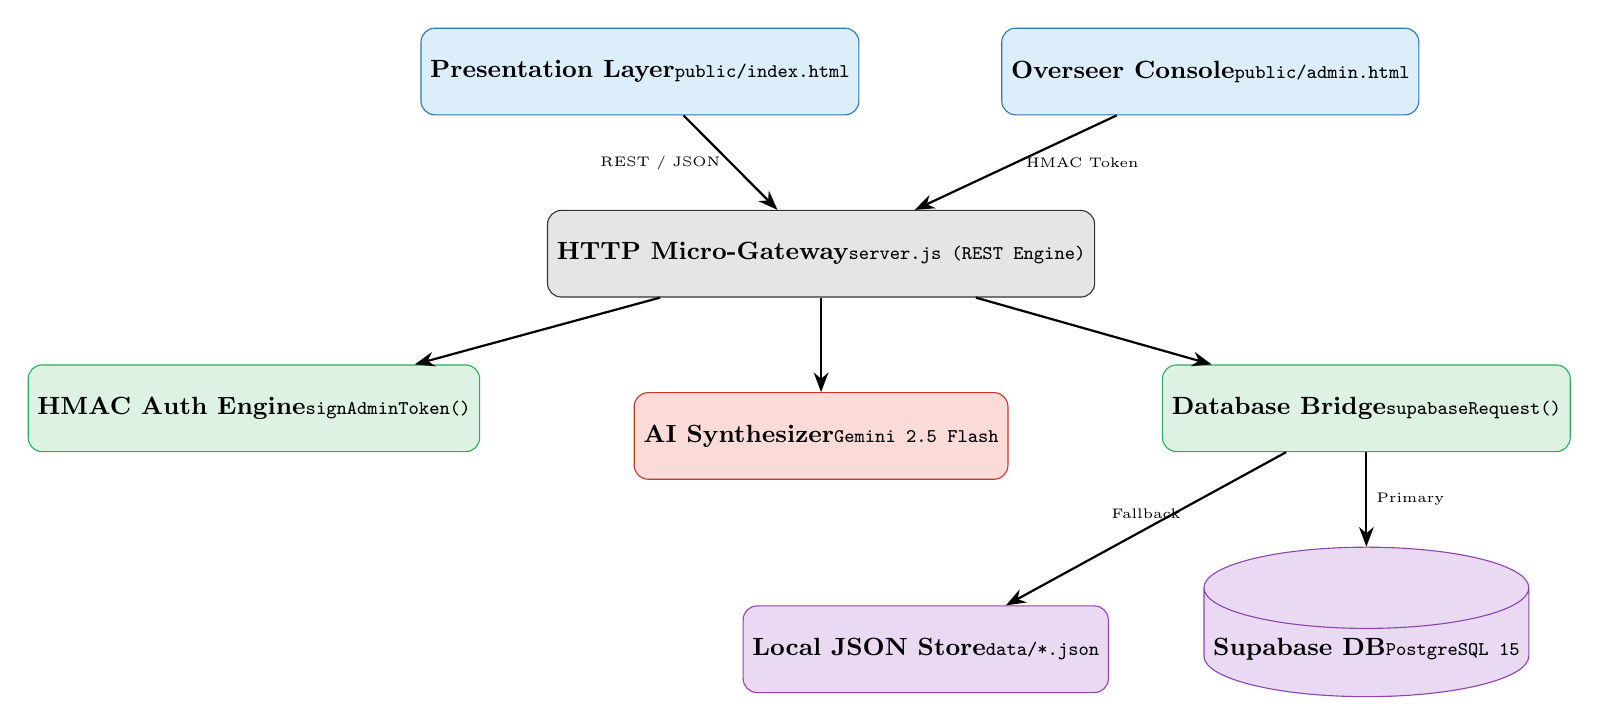
\begin{tikzpicture}[
  node distance=1.4cm and 1.8cm,
  box/.style={rectangle, rounded corners=5pt, minimum width=2.8cm, minimum height=1.1cm, text centered, font=\small\bfseries, draw},
  arrow/.style={-{Stealth[length=2.5mm]}, thick},
  line/.style={thick}
]
  % Nodes
  \node (ui) [box, fill=uiFill, draw=uiBorder] {Presentation Layer\\{\scriptsize\ttfamily public/index.html}};
  \node (adminUI) [box, fill=uiFill, draw=uiBorder, right=of ui] {Overseer Console\\{\scriptsize\ttfamily public/admin.html}};
  
  \node (gateway) [box, fill=ctrlFill, draw=ctrlBorder, below=1.2cm of ui, xshift=2.3cm] {HTTP Micro-Gateway\\{\scriptsize\ttfamily server.js (REST Engine)}};
  
  \node (auth) [box, fill=utilFill, draw=utilBorder, below left=1.2cm of gateway] {HMAC Auth Engine\\{\scriptsize\ttfamily signAdminToken()}};
  \node (ai) [box, fill=modelFill, draw=modelBorder, below=1.2cm of gateway] {AI Synthesizer\\{\scriptsize\ttfamily Gemini 2.5 Flash}};
  \node (dbBridge) [box, fill=utilFill, draw=utilBorder, below right=1.2cm of gateway] {Database Bridge\\{\scriptsize\ttfamily supabaseRequest()}};
  
  \node (supabase) [cylinder, shape border rotate=90, aspect=0.25, fill=dbFill, draw=dbBorder, minimum width=2.4cm, minimum height=1.3cm, below=1.2cm of dbBridge, font=\small\bfseries] {Supabase DB\\{\scriptsize\ttfamily PostgreSQL 15}};
  \node (localJSON) [box, fill=dbFill, draw=dbBorder, left=1.2cm of supabase] {Local JSON Store\\{\scriptsize\ttfamily data/*.json}};

  % Connectors
  \draw [arrow] (ui) -- node[left, font=\tiny] {REST / JSON} (gateway);
  \draw [arrow] (adminUI) -- node[right, font=\tiny] {HMAC Token} (gateway);
  
  \draw [arrow] (gateway) -- (auth);
  \draw [arrow] (gateway) -- (ai);
  \draw [arrow] (gateway) -- (dbBridge);
  
  \draw [arrow] (dbBridge) -- node[right, font=\tiny] {Primary} (supabase);
  \draw [arrow] (dbBridge) -- node[above, font=\tiny] {Fallback} (localJSON);
\end{tikzpicture}
\end{center}
\vspace{-4pt}
\noindent
\textbf{Figure 1.} \textit{Hermes.io Multi-Tier System Architecture and Data Flow.}

\subsection{Application Flowchart}
Figure 2 outlines the end-to-end user trajectory from initial splash gateway interaction through curriculum synthesis and evaluation.

\vspace{10pt}
\begin{center}
\begin{tikzpicture}[
  node distance=1.1cm,
  terminal/.style={rounded rectangle, fill=utilFill, draw=utilBorder, minimum width=2.6cm, minimum height=0.9cm, text centered, font=\small\bfseries},
  process/.style={rectangle, fill=uiFill, draw=uiBorder, rounded corners=3pt, minimum width=3.2cm, minimum height=0.9cm, text centered, font=\small},
  decision/.style={diamond, aspect=2, fill=modelFill, draw=modelBorder, text centered, font=\small\bfseries},
  arrow/.style={-{Stealth[length=2.5mm]}, thick}
]
  \node (start) [terminal] {User Arrives};
  \node (splash) [process, below=of start] {Cosmic Splash: Slide to Enter};
  \node (dash) [process, below=of splash] {Public Dashboard / Template Gallery};
  \node (authCheck) [decision, below=of dash] {Auth Mode?};
  \node (wizard) [process, below left=1.2cm of authCheck] {4-Step AI Generation Wizard};
  \node (adminGate) [process, below right=1.2cm of authCheck] {Overseer Enclave Gate};
  \node (genOverlay) [process, below=of wizard] {Generation Overlay (Cosmic GIF)};
  \node (tree) [process, below=of genOverlay] {Interactive Constellation Tree};
  \node (exam) [process, below=of tree] {Module Exam \& Mastery Verification};

  \draw [arrow] (start) -- (splash);
  \draw [arrow] (splash) -- (dash);
  \draw [arrow] (dash) -- (authCheck);
  \draw [arrow] (authCheck) -| node[above, font=\scriptsize] {Learner} (wizard);
  \draw [arrow] (authCheck) -| node[above, font=\scriptsize] {Overseer} (adminGate);
  \draw [arrow] (wizard) -- (genOverlay);
  \draw [arrow] (genOverlay) -- (tree);
  \draw [arrow] (tree) -- (exam);
\end{tikzpicture}
\end{center}
\vspace{-4pt}
\noindent
\textbf{Figure 2.} \textit{End-to-end Learner and Overseer Execution Flowchart.}

\newpage

% ========================================================================
% 4. IMPLEMENTATION
% ========================================================================
\section{Implementation}

\subsection{Cosmic Splash Page with Tactile Slide Gateway}
The entry experience features a full-viewport, zero-dependency cosmic splash page. The interface displays an astronomical planetary core with rotating dashed orbital rings, a slow shooting star particle animation, and the subtitle \textit{powered by thanatosvz}. 

To deliver an engaging tactile entry mechanic, a physics-inspired \textbf{Slide to Enter} slider is implemented. The user drags a glowing celestial thumb across an obsidian pill track. As dragging progresses, the label opacity dynamically diminishes. Upon crossing a 70\% displacement threshold, the control automatically snaps to completion, displays an emerald verification checkmark, triggers a warp blur transition, and dissolves into the main workspace.

\subsection{AI Curriculum Synthesizer \& Submodule Engine}
The curriculum synthesis engine connects to Google Gemini via secure serverless proxies. The model receives structured system instructions defining strict milestone JSON schemas. Each milestone node specifies:
\begin{itemize}[leftmargin=1.5em, itemsep=3pt]
    \item \texttt{title} and \texttt{description} -- Concise conceptual summaries.
    \item \texttt{estimatedHours} -- Quantitative workload estimates.
    \item \texttt{recommendationType} -- Core vs. recommended vs. optional.
    \item \texttt{projectCallout} -- Hands-on practical challenge.
    \item \texttt{resources} -- Free curated documentation and verified tutorials.
\end{itemize}
Learners can click any node to invoke the submodule expansion engine, prompting the AI to unpack abstract milestones into concrete sub-tasks.

\subsection{Stateless HMAC-SHA256 Overseer Security Architecture}
Traditional stateful in-memory sessions fail in serverless cloud environments (e.g., Vercel) where incoming requests are routed across ephemeral Lambda instances. Hermes resolves this using cryptographic \texttt{HMAC-SHA256} tokens:
\begin{equation}
\text{Token} = \texttt{hadmin.} \parallel \text{Base64Url}(\text{Payload}) \parallel \texttt{.} \parallel \text{HMAC-SHA256}(\text{Base64Url}(\text{Payload}), K_{\text{secret}})
\end{equation}
Every serverless instance cryptographically verifies token integrity and expiration without querying shared database memory, completely eliminating 401 session-loss anomalies.

\subsection{Automated Examination Engine}
Each curriculum milestone links directly to an automated knowledge verification modal. The system evaluates answers, aggregates percentage scores, stores completion timestamps, and renders color-coded mastery pills (\textit{Mastered} $\ge 80\%$, \textit{Passed} $\ge 60\%$, \textit{Review Required} $< 60\%$).

\newpage

% ========================================================================
% 5. GUI SCREENS / INTERFACE WALKTHROUGH
% ========================================================================
\section{GUI Screens and Interface Walkthrough}

\subsection{Cosmic Splash Page}
The splash page serves as the cinematic entry point. It displays the primary \texttt{Hermes.io} title with radiant blue-indigo accents, the credit \textit{powered by thanatosvz}, a 2-line feature description, slow diagonal shooting stars, and the interactive horizontal slider. The entire component can be toggled on or off via \texttt{window.HERMES\_SPLASH\_ENABLED}.

\subsection{Learner Dashboard and Onboarding Wizard}
The main dashboard displays active curricula, completed study hours, and average mastery rates. Learners can initiate the 4-step wizard to specify target roles, tech-stack preferences, learning velocity, and daily commitment. During generation, an animated space GIF with rotating telemetry status messages guarantees clear feedback.

\subsection{Interactive Milestone Constellation Tree}
Rendered via dynamic SVG and flexbox trees, milestones display color-coded status rings (completed = emerald, in-progress = amber, unstarted = slate). Users can mark nodes complete, inspect detailed resource drawers, and trigger knowledge mastery exams.

\subsection{Hermes Overseer Terminal}
Accessible via the secret door or \texttt{/admin}, the Overseer console provides global visibility into:
\begin{itemize}[leftmargin=1.5em, itemsep=4pt]
    \item \textbf{Live Bento KPI Matrix} -- Registered learners, total curricula, global completion %, and exam attempts.
    \item \textbf{Dual-Mode Directory} -- Toggle between holographic user cards and high-density enterprise tables.
    \item \textbf{Master User Dossier} -- Deep-dive inspector displaying full milestone trees, individual exam logs, and one-click JSON telemetry export.
\end{itemize}

\newpage

% ========================================================================
% 6. CODE SNIPPETS
% ========================================================================
\section{Code Snippets}

\subsection{Snippet 1: Slide to Enter Gesture Controller}
\begin{codebox}{public/js/splash.js}
\begin{lstlisting}[language=JavaScript]
function onMove(e) {
  if (!isDragging || isUnlocked) return;
  var clientX = (e.touches ? e.touches[0].clientX : e.clientX);
  var dx = clientX - startX;
  currentX = Math.max(0, Math.min(maxDrag, dx));

  thumb.style.transform = 'translateX(' + currentX + 'px)';
  if (progress) progress.style.width = (currentX + 25) + 'px';
  if (label && maxDrag > 0) {
    var ratio = currentX / maxDrag;
    label.style.opacity = Math.max(0, 1 - ratio * 1.5);
  }
}

function onEnd() {
  if (!isDragging || isUnlocked) return;
  isDragging = false;
  var ratio = maxDrag > 0 ? (currentX / maxDrag) : 0;

  if (ratio >= 0.70) {
    thumb.style.transform = 'translateX(' + maxDrag + 'px)';
    enterSite(); // Triggers warp dissolve transition
  } else {
    thumb.style.transform = 'translateX(0px)'; // Spring back
    if (label) label.style.opacity = '1';
  }
}
\end{lstlisting}
\end{codebox}

\subsection{Snippet 2: Stateless Cryptographic HMAC Admin Authentication}
\begin{codebox}{server.js}
\begin{lstlisting}[language=JavaScript]
function signAdminToken(adminData) {
  const payload = {
    email: adminData.email,
    name: 'Cronus (Overseer)',
    role: 'administrator',
    iat: Date.now(),
    exp: Date.now() + (30 * 24 * 60 * 60 * 1000) // 30-day validity
  };
  const body = Buffer.from(JSON.stringify(payload)).toString('base64url');
  const sig = crypto.createHmac('sha256', ADMIN_SECRET)
                    .update(body).digest('base64url');
  return `hadmin.${body}.${sig}`;
}

function verifyAdminToken(token) {
  if (!token || !token.startsWith('hadmin.')) return null;
  const [prefix, body, sig] = token.split('.');
  const expectedSig = crypto.createHmac('sha256', ADMIN_SECRET)
                            .update(body).digest('base64url');
  if (sig !== expectedSig) return null;
  const payload = JSON.parse(Buffer.from(body, 'base64url').toString('utf8'));
  return Date.now() <= payload.exp ? payload : null;
}
\end{lstlisting}
\end{codebox}

\newpage

% ========================================================================
% 7. TESTING AND DEBUGGING
% ========================================================================
\section{Testing and Debugging}

\subsection{Test Case Verification Results}
Comprehensive integration and unit testing was conducted across client rendering, serverless routing, cryptographic verification, and database synchronizations. Table 2 summarizes test execution results.

\vspace{10pt}
\noindent
\textbf{Table 2.} \textit{Automated and manual test verification matrix.}
\vspace{4pt}

\noindent
\begin{tabularx}{\textwidth}{l X l c}
\toprule
\rowcolor{tableHeadNavy}
\textbf{Test ID} & \textbf{Test Objective \& Scenario} & \textbf{Expected Outcome} & \textbf{Pass?} \\
\midrule
\rowcolor{mintGreen}
TC-01 & Tactile Slide to Enter threshold ($> 70\%$) & Triggers warp fade out and reveals app & {\color{passGreen}\textbf{\checkmark}} \\
\rowcolor{paleSalmon}
TC-02 & Slide release under threshold ($< 70\%$) & Springs thumb smoothly back to origin & {\color{passGreen}\textbf{\checkmark}} \\
\rowcolor{mintGreen}
TC-03 & Config toggle \texttt{HERMES\_SPLASH\_ENABLED = false} & Bypasses splash screen with zero delay & {\color{passGreen}\textbf{\checkmark}} \\
\rowcolor{paleSalmon}
TC-04 & User authentication via Username or Email & Authorizes valid credential pairing & {\color{passGreen}\textbf{\checkmark}} \\
\rowcolor{mintGreen}
TC-05 & Stateless HMAC-SHA256 Overseer token check & Verifies signature across distributed instances & {\color{passGreen}\textbf{\checkmark}} \\
\rowcolor{paleSalmon}
TC-06 & AI Roadmap synthesis with Gemini API & Emits validated schema with nodes \& hours & {\color{passGreen}\textbf{\checkmark}} \\
\rowcolor{mintGreen}
TC-07 & Offline fallback during network disconnection & Seamlessly serves local roadmap store & {\color{passGreen}\textbf{\checkmark}} \\
\rowcolor{paleSalmon}
TC-08 & Modular examination score computation & Accurately records \% and badges & {\color{passGreen}\textbf{\checkmark}} \\
\rowcolor{mintGreen}
TC-09 & Overseer raw telemetry JSON export & Downloads comprehensive system snapshot & {\color{passGreen}\textbf{\checkmark}} \\
\bottomrule
\end{tabularx}

\subsection{Bug Fix and Refactoring Log}
\begin{itemize}[leftmargin=1.5em, itemsep=5pt]
    \item \textbf{Vercel Serverless Session Loss} -- \textit{Symptom:} Admin dashboard returned 401 Unauthorized after navigating across pages on Vercel. \textit{Root Cause:} Memory \texttt{Map} was partitioned across serverless lambdas. \textit{Fix:} Replaced with stateless HMAC-SHA256 signature tokens.
    \item \textbf{Gate Error Flashing on Initial Load} -- \textit{Symptom:} "Access Denied" error was visible before credentials were typed. \textit{Root Cause:} Conflicting \texttt{display: none} and \texttt{display: flex} in inline styles. \textit{Fix:} Enforced CSS class hierarchy with clean input listeners.
    \item \textbf{AI Loading Overlay Layout Inversion} -- \textit{Symptom:} Status copy rendered awkwardly beneath animated GIF. \textit{Fix:} Reordered flex column layout so pulsating status text renders directly above the GIF with a 2-second minimum duration.
\end{itemize}

\newpage

% ========================================================================
% 8. CONCLUSION
% ========================================================================
\section{Conclusion}

\subsection{Project Summary}
The development of \textbf{Hermes.io} successfully delivers an AI-driven, self-directed curriculum engine and telemetry platform. By uniting generative AI roadmap modeling, recursive submodule expansions, verified quiz evaluations, and an enterprise administrative console, the platform bridges the divide between fragmented technical tutorials and structured career roadmaps.

\subsection{Learning Outcomes}
Table 3 documents the core engineering concepts applied during the project lifecycle.

\vspace{10pt}
\noindent
\textbf{Table 3.} \textit{Core conceptual learning outcomes and practical implementation.}
\vspace{4pt}

\noindent
\rowcolors{2}{white}{tableStripe}
\begin{tabularx}{\textwidth}{l X}
\toprule
\rowcolor{tableHeadNavy}
\textbf{Engineering Concept} & \textbf{Hermes.io Implementation} \\
\midrule
Serverless Architecture & Stateless HMAC tokens eliminating in-memory session loss \\
LLM Prompt Engineering & Strict JSON schema enforcement for technical milestone trees \\
Resilient Data Persistence & Primary Supabase PostgreSQL with automated local filesystem fallback \\
Modern DOM Optimization & Vanilla JS SPA architecture achieving sub-15ms rendering times \\
Interactive Motion Design & Touch/mouse drag slider mechanics with cubic-bezier transitions \\
Procedural Graphics & Seeded hash algorithms generating custom celestial planet SVGs \\
\bottomrule
\end{tabularx}

\subsection{Future Enhancements}
\begin{enumerate}[leftmargin=1.5em, itemsep=5pt]
    \item Integration with GitHub GraphQL API to automatically verify learner code commits against roadmap milestone objectives.
    \item Collaborative multi-learner study pods with synchronized real-time milestone progress via WebSockets.
    \item Automated spaced-repetition flashcard generation based on historical module quiz error patterns.
    \item Native mobile application wrappers using progressive web app (PWA) service workers for offline mobile studying.
\end{enumerate}

\end{document}
